\section{Method}
\label{sec:method}
\subsection{Overview}

UrbanDreamer follows the world-model formulation of
Section~\ref{sec:wm-formulation}, alternating real and imagined transitions:
\begin{enumerate}
  \item \textbf{Collect.}
  The current actor routes the CAVs in the simulator; the episode is stored
  in a replay buffer with the sampled routes and the observed HDV pattern.

  \item \textbf{Fit.}
  The world model and the HDV response predictor are updated on replay
  transitions, giving the learned transition
  \(\hat Z_{t+1}=F_\phi(Z_t;C_t)\) with
  \(C_t=(\Psi_t^{\mathrm{CAV}},D_t,\hat H^{\mathrm{HDV}})\).

  \item \textbf{Imagine.}
  From a replay state, the actor samples routes, the pressure
  \(\Psi_t^{\mathrm{CAV}}\) conditions the world model, and a vehicle wrapper
  advances each CAV along its route under the decoded travel times.

  \item \textbf{Optimize.}
  Imagined rewards form per-vehicle and global returns that update the actor
  and both critics. Saved actors are evaluated in the simulator, and the
  final converged checkpoint is reported.
\end{enumerate}



\begin{figure*}[t]
  \centering
  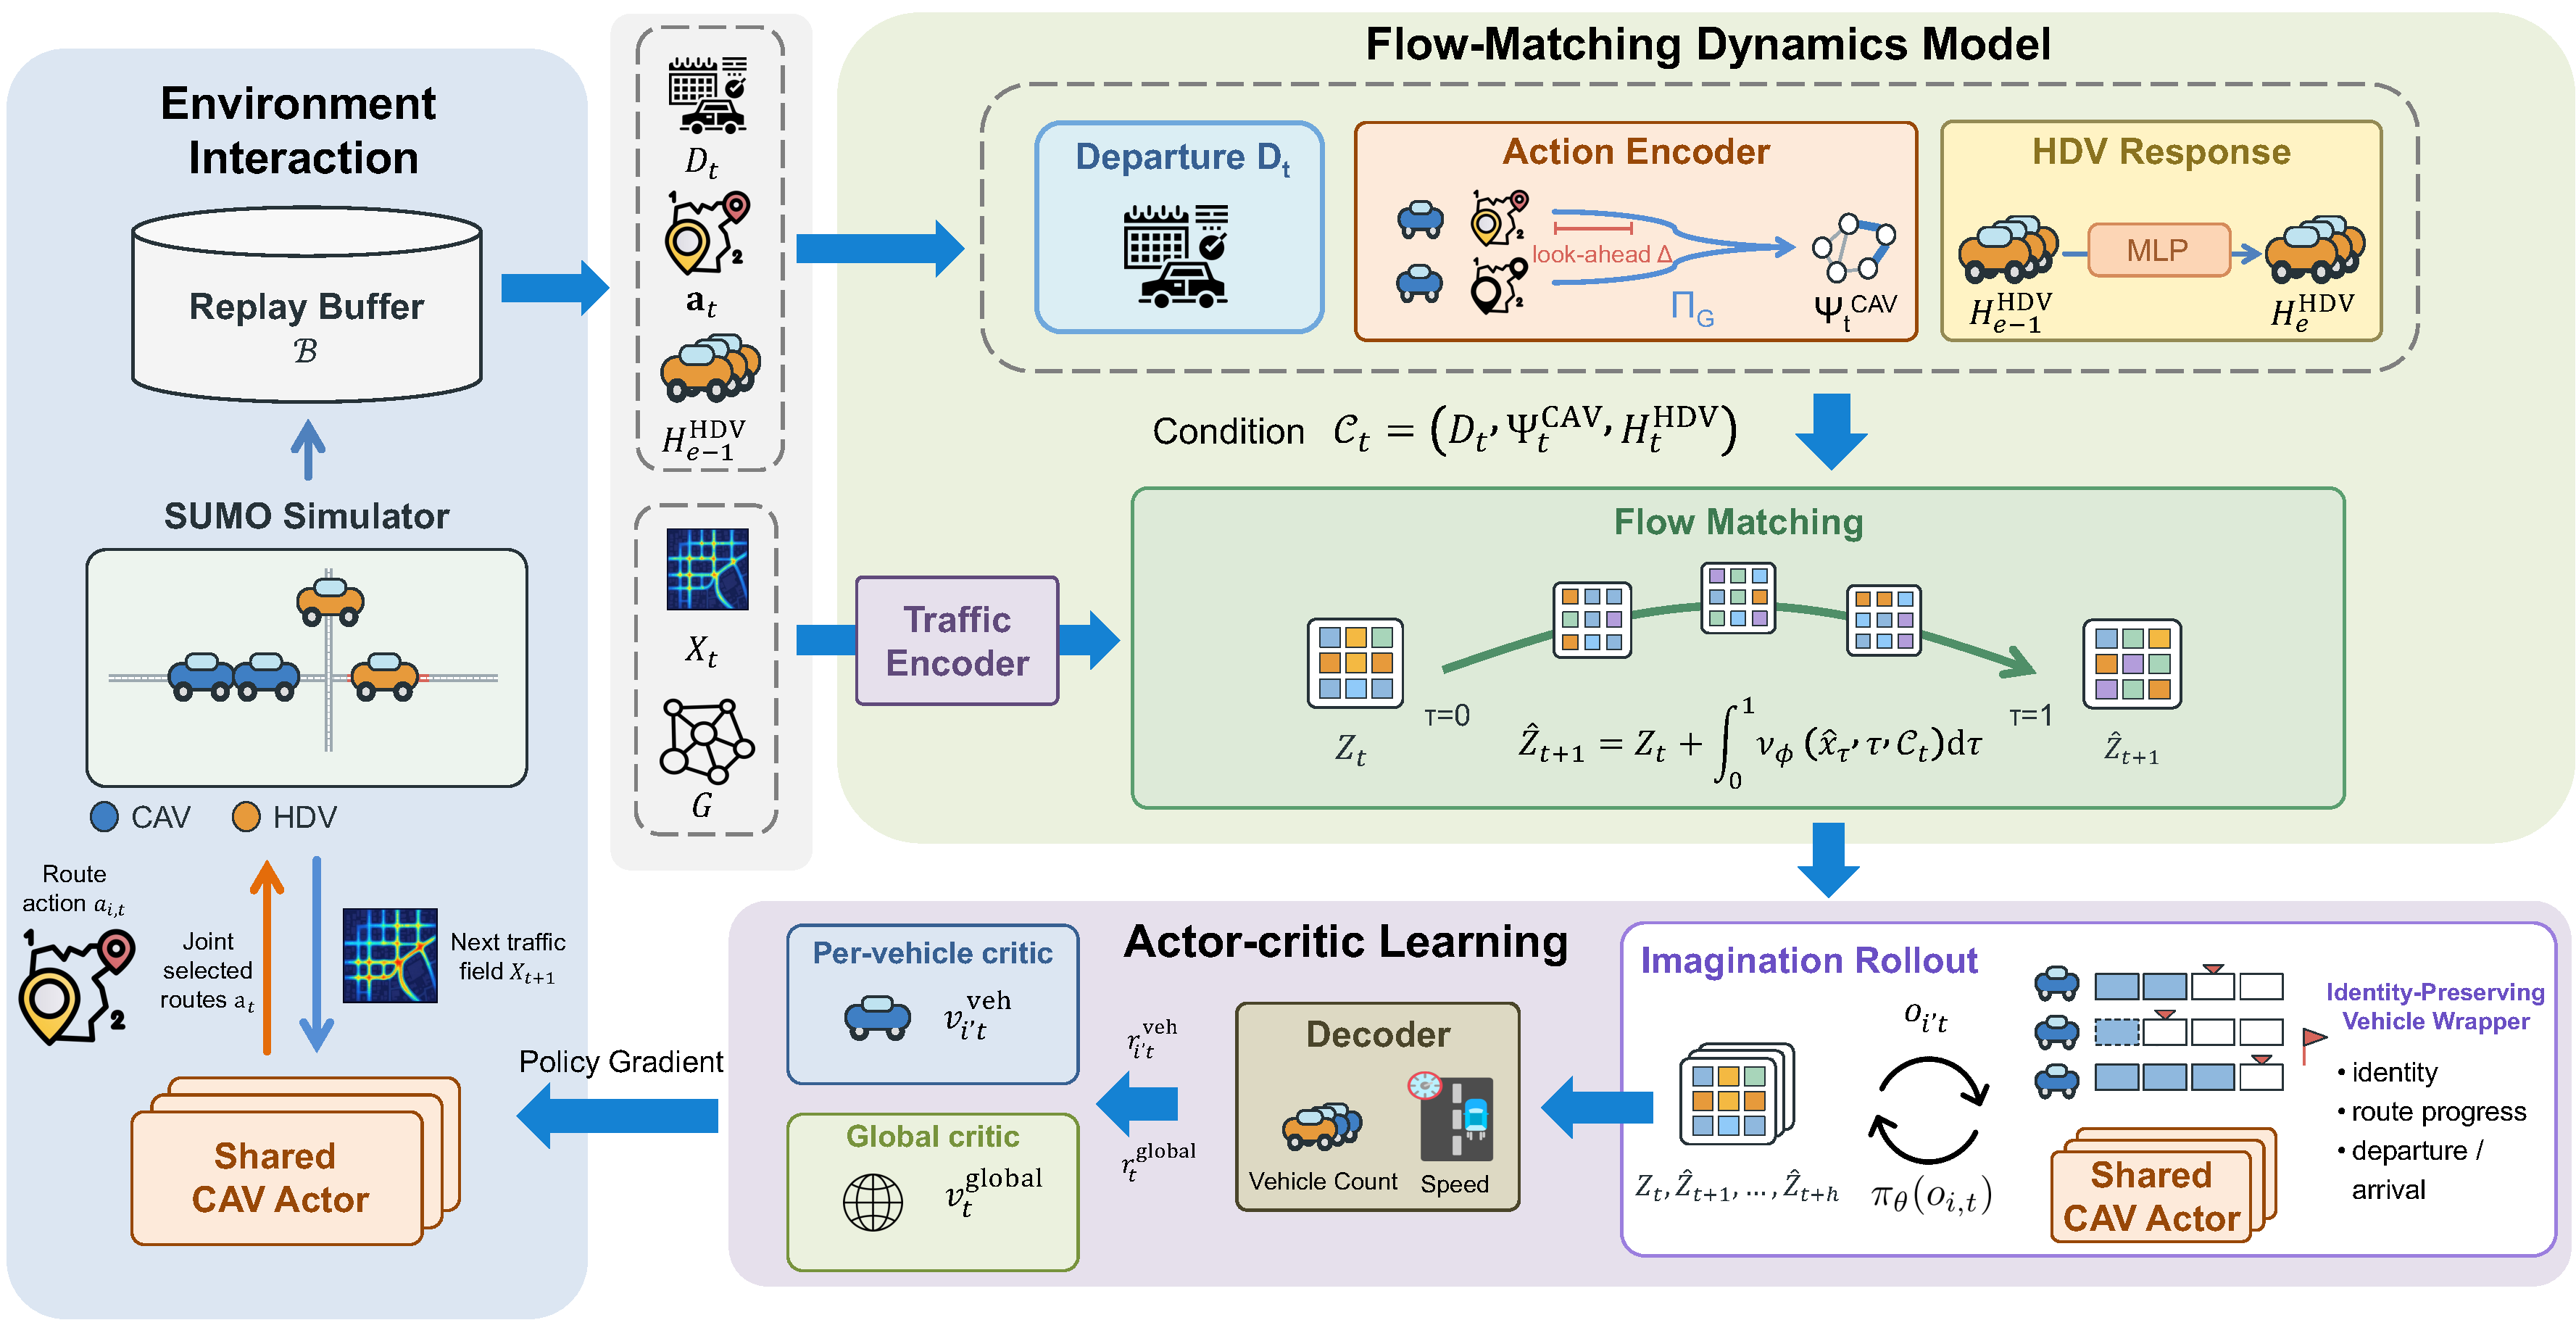
\includegraphics[width=0.8\textwidth]{figure/UrbanDreamer}
  \caption{Overview of UrbanDreamer.}
  \label{fig:architecture}
\end{figure*}


\subsection{Flow Matching Dynamics Model}


\subsubsection{Traffic Encoder and Decoder}

A stack of graph convolution layers with residual connections and layer
normalization maps the traffic field \(X_t\) to the latent representation
\(Z_t\), whose row \(z_{t,u}\) summarizes segment \(u\) together with its
graph neighborhood (Appendix~\ref{app:math-details}).  A decoder maps each
\(z_{t,u}\) back to the dynamic segment attributes
\([\hat c_{t,u},\hat v_{t,u}]\), trained jointly with the dynamics model
through a reconstruction loss on observed traffic fields, and provides the
travel-time and count readouts for rewards and value targets in actor-critic
learning.


\subsubsection{Action Encoder}

The transition model evolves graph-level representations, but decisions are
made at the vehicle level.  We therefore project the realized one-hot CAV
route decisions onto the segment nodes those routes are expected to visit,
producing a planned pressure field \(\Psi_t^{\mathrm{CAV}}\) defined on the
same segment set as \(X_t\) and \(Z_t\).  For active CAV \(i\), let
\(\mathrm{Seg}_{\Delta}(P^k_{i,t})\subseteq N\) denote the segments it would
enter within the look-ahead window \(\Delta\) under candidate \(P^k_{i,t}\);
the planned pressure averages route indicators over the active set:
\begin{equation}
\begin{array}{rcl}
\Psi_t^{\mathrm{CAV}}(u)
=
\displaystyle
\frac{1}{\max(|\mathcal{I}_t|,1)}
\sum_{i\in\mathcal{I}_t}\sum_{k=1}^{K}
\mathbf{1}[k=a_{i,t}]
\displaystyle
\,\xi_{i,t}^{k,\Delta}(u),\\
\xi_{i,t}^{k,\Delta}(u)
=
\left\{
\begin{array}{ll}
1, & u\in\mathrm{Seg}_{\Delta}(P^k_{i,t})\\
0, & \mathrm{otherwise}
\end{array}
\right.
\end{array}
\end{equation}
The same sampled one-hot route is executed by the vehicle, stored in replay,
and supplied to the transition condition, so \(\Psi_t^{\mathrm{CAV}}\)
always matches the physical intervention.  The mean normalization states
where the controlled demand intends to go, not how large it is.



\subsubsection{State-to-State Flow Matching}

UrbanDreamer learns the latent transition with state-to-state flow
matching \cite{GiFlow} under the transition condition
\begin{equation}
\mathcal{C}_t=
(\Psi_t^{\mathrm{CAV}},D_t,H_t^{\mathrm{HDV}}).
\end{equation}
Instead of regressing \(Z_{t+1}\) directly, the model learns a velocity
field that transports the current latent representation to the next one.
For a real transition pair \((Z_t,Z_{t+1})\), sample
\(\tau\sim\mathcal{U}(0,1)\) and define
\begin{equation}
\begin{array}{rcl}
x_\tau &=& (1-\tau)Z_t+\tau Z_{t+1},\\
\nu_{t,\tau} &=& \frac{dx_\tau}{d\tau} = Z_{t+1}-Z_t.
\end{array}
\end{equation}
The previous latent representation \(Z_t\) is the flow source, and
\(\nu_{t,\tau}\) is the target velocity.  This deterministic state-to-state
transport is based on rectified flow \cite{lipman2023flow,liu2023rectified}:
the straight interpolation path keeps multi-step imagined rollouts stable,
and we do not claim multimodal generative modeling of \(Z_{t+1}\).

We parameterize the velocity predictor \(\nu_\phi\) with a block-causal
transformer \cite{vaswani2017attention} over segment traffic
representations, which receives the interpolated representation \(x_\tau\),
the time condition \(\tau\), and the transition condition \(\mathcal{C}_t\),
mixes information through causal attention over previous traffic
representations, and outputs the velocity estimate
\begin{equation}
\hat\nu_{t,\tau}=\nu_\phi(x_\tau,\tau,\mathcal{C}_t).
\end{equation}
Because most road segments are empty most of the time, the training loss
applies bounded per-segment weights \(w_{t,u}\) that emphasize occupied and
congested segments (Appendix~\ref{app:math-details}).

At imagination time, the next latent traffic representation is obtained by
integrating the learned velocity field with \(k\) explicit Euler steps:
\begin{equation}
\begin{array}{rcl}
\hat Z_{t+1}
&=&
\displaystyle
Z_t+\int_0^1
\nu_\phi(\hat x_\tau,\tau,\mathcal{C}_t)\,d\tau.
\end{array}
\end{equation}
Multi-step imagination repeatedly applies this one-step transition, using
each predicted \(\hat Z_{t+1}\) as the next source representation.
% 中文注释：想象阶段从 \(x_0=Z_t\) 对速度场做 ODE 积分；多步想象反复应用一步 transition。


\subsection{HDV Response Module}

HDVs choose routes at departure time and adapt across episodes to the
congestion that CAV routing induces.  UrbanDreamer models the two time
scales separately.  Within an episode, the learned transition responds to
the current CAV pressure \(\Psi_t^{\mathrm{CAV}}\) at every decision epoch.
Across episodes, slower human adaptation is represented as an episode-level
response field over road segments, predicted from the previous episode and
held fixed within each imagined episode.  Imagined rollouts therefore
optimize against step-level counterfactual traffic responses, while
day-to-day HDV demand shifts are learned from real simulator episodes
rather than simulated inside imagination.

The HDV influence is represented as a road-segment distribution
\(H^{\mathrm{HDV}}\): the supervision target \(H^\star\) aggregates the
observed HDV background field over an episode and normalizes it across
segments, and an MLP with a softmax output estimates
\(\hat H_e^{\mathrm{HDV}}\) from the previous episode's CAV pressure summary
and HDV background.  The predictor is trained with a soft-label
cross-entropy loss and an optimizer separate from the world model, so HDV
adaptation is learned without treating HDVs as controllable
(Appendix~\ref{app:math-details}).




\subsection{Actor-Critic Learner}

The learner runs the following loop inside the learned model.  An imagined
rollout is generated by the actor, the world model, and a vehicle wrapper;
each imagined step produces a per-vehicle travel-time reward and a
network-level global reward; two centralized critics estimate the
corresponding returns; and the actor is updated from their combined
advantage.  This dense credit is necessary because the global mean travel
time in Definition~7 is an episode-level objective that is available only
after a simulator episode is completed.  The per-vehicle signal is the
primary actor-learning signal, while the global critic supplies an auxiliary
aggregate value signal.
% 中文注释：学习循环：actor、world model 和 vehicle wrapper 生成 imagined rollout；每个 imagined step 产生 per-vehicle travel-time reward 和 network-level global reward；两个 centralized critics 估计对应 returns;actor 用组合 advantage 更新。需要 dense credit 是因为 Definition~7 的 global mean travel time 是 episode 级目标，只有 simulator episode 完成后才能获得。per-vehicle signal 是主要 actor-learning signal,global critic 提供辅助的 aggregate value signal。

\subsubsection{Vehicle-Level Imagination}

Imagined rollouts start from a replay state: we sample a replay episode and a
decision epoch \(t_{\mathrm{start}}\), encode the aligned traffic field as
\(Z_{t_{\mathrm{start}}}=f_\phi(X_{t_{\mathrm{start}}},G)\), and initialize
each vehicle's current segment, destination, route suffix, and arrival status
from the same epoch.  At each imagined epoch, the actor selects a route and
the decoder recovers the segment speed \(\widehat v_{t,u}\), giving the
predicted segment travel time
\begin{equation}
\begin{array}{rcl}
\widehat\tau_t(u)
&=&
\displaystyle
\frac{\ell(u)}{\widehat v_{t,u}}.
\end{array}
\end{equation}
During a decision interval \(\Delta t\), a deterministic vehicle wrapper
advances each vehicle along its selected route by consuming these travel times
in route order, while the learned transition predicts \(Z_{t+1}\).  Because
the wrapper and the transition consume the same decoded readout, vehicle
positions and the segment traffic field evolve from a single prediction rather
than two independent state estimates.  Vehicles reaching their departure time
are added at the next epoch and arrived vehicles are removed; the remaining
CAVs form \(\mathcal{I}_{t+1}^{\mathrm{im}}\) and alone contribute actor
samples, rewards, and bootstrap values.  This wrapper keeps vehicle identity
explicit without requiring the graph-level world model to predict per-vehicle
terminal variables.
% 中文注释：imagined rollout 从 replay state 初始化：采样 replay episode 和 decision epoch \(t_{\mathrm{start}}\)，编码 \(Z_{t_{\mathrm{start}}}=f_\phi(X_{t_{\mathrm{start}}},G)\)，并从同一 epoch 初始化每辆车的 current segment、destination、route suffix 和 arrival status。每个 imagined epoch,actor 选择 route,decoder 给出 segment speed \(\widehat v_{t,u}\) 和 travel time \(\widehat\tau_t(u)=\ell(u)/\widehat v_{t,u}\)。deterministic vehicle wrapper 在 \(\Delta t\) 内按 route 顺序消耗这些 travel time 推进车辆，同时 transition 预测 \(Z_{t+1}\);wrapper 与 transition 共享同一 decoded readout，因此车辆位置与 segment field 来自同一个预测。到点车辆加入、到达车辆移除，剩余 CAV 构成 \(\mathcal{I}_{t+1}^{\mathrm{im}}\)。该 wrapper 在不要求 world model 预测 per-vehicle terminal variables 的情况下显式保留 vehicle identity。

\subsubsection{Imagined Rewards}

For the route selected by CAV \(i\), let \(P_{i,t}^{\mathrm{rem}}\) denote its
suffix road segments.  The per-vehicle reward charges the imagined travel time
accumulated before the next decision or arrival:
\begin{equation}
\begin{array}{rcl}
\widehat T_{i,t}^{\mathrm{rem}}
&=&
\displaystyle
\sum_{u\in P_{i,t}^{\mathrm{rem}}}
\widehat\tau_{t+1}(u),\\[0.35em]
\delta_{i,t}
&=&
\min(\Delta,\widehat T_{i,t}^{\mathrm{rem}}),\\
r_{i,t}^{\mathrm{veh}}
&=&
-\delta_{i,t}/\kappa_r,
\end{array}
\end{equation}
where \(\kappa_r\) controls the reward scale.
% 中文注释：per-vehicle reward 由 \(\delta_{i,t}=\min(\Delta,\widehat T_{i,t}^{\mathrm{rem}})\) 和 \(r_{i,t}^{\mathrm{veh}}=-\delta_{i,t}/\kappa_r\) 给出，其中 \(\widehat T_{i,t}^{\mathrm{rem}}\) 是所选 route 剩余 suffix 的 predicted travel time。

The global reward charges each decision interval by the travel time
accumulated by all vehicles present in the network:
\begin{equation}
\begin{array}{rcl}
r_t^{\mathrm{global}}
&=&
\displaystyle
-\kappa_g\,
\frac{N_{\mathrm{active}}(t)\,\Delta t}{N_{\mathrm{veh}}},
\end{array}
\end{equation}
where \(N_{\mathrm{veh}}\) is the episode vehicle population and \(\kappa_g\)
controls the reward scale.  On real transitions, \(N_{\mathrm{active}}(t)\) is
read directly from the simulator state.  In imagined rollouts, it is computed
from the decoded count field, \(N_{\mathrm{active}}(t)=\sum_{u\in N}\widehat
n_{t,u}\) with \(\widehat n_{t,u}=\kappa(u)\hat c_{t,u}\).  Since \(\sum_t
N_{\mathrm{active}}(t)\Delta t\) is the total travel time accumulated over an
episode, the sum of \(r_t^{\mathrm{global}}\) equals \(-\kappa_g\) times the
global mean travel time of Definition~7.  Both rewards are therefore computed
from the decoded readouts rather than learned.
% 中文注释：global reward 按当前网络中所有车辆累计的通行时间对每个 decision interval 计费：\(r_t^{\mathrm{global}}=-\kappa_g N_{\mathrm{active}}(t)\Delta t/N_{\mathrm{veh}}\)。真实 transition 上 \(N_{\mathrm{active}}(t)\) 直接从 simulator 读取；imagined rollout 中用 decoded count field 求和 \(\sum_u\widehat n_{t,u}\),\(\widehat n_{t,u}=\kappa(u)\hat c_{t,u}\)。由于 \(\sum_t N_{\mathrm{active}}(t)\Delta t\) 是整个 episode 累计的总通行时间，\(r_t^{\mathrm{global}}\) 的求和等于 \(-\kappa_g\) 倍的 Definition~7 global mean travel time。两种 reward 都由 decoded readouts 计算得到，不需要学习。

\subsubsection{Critics}

The per-vehicle critic first encodes every observation independently with a
parameter-shared multilayer perceptron (MLP) \(f_\eta^{\mathrm{enc}}\), and then
applies multi-head self-attention within the active CAV set:
\begin{equation}
\begin{array}{rcl}
e_{i,t} &=& f_\eta^{\mathrm{enc}}(o_{i,t}),\\
(\widetilde e_{i,t})_{i\in\mathcal{I}_t}
&=&
\mathrm{Attention}_\eta((e_{i,t})_{i\in\mathcal{I}_t}),\\
v_{i,t}^{\mathrm{veh}}
&=&
w_v^\top\widetilde e_{i,t}+b_v.
\end{array}
\end{equation}
The attention layer lets each value estimate account for simultaneous CAV
decisions and route overlap, while \(v_{i,t}^{\mathrm{veh}}\) remains a
per-vehicle estimate of the future return.  It is trained by lambda returns
linked by vehicle identity: only observations of the same CAV are connected by
the recursion, and bootstrapping stops once the vehicle leaves the active set
(Appendix~\ref{app:math-details}).
% 中文注释：per-vehicle critic 先用 parameter-shared MLP 独立编码每个 observation，再在 active CAV set 内做 multi-head self-attention，使每个 value 能考虑 simultaneous decisions 和 route overlap，但仍为每辆车输出一个 value。它用按 vehicle identity 连接的 lambda returns 训练；车辆离开 active set 后停止 bootstrap。

The auxiliary global critic reuses the graph representation \(\bar z_t\):
\begin{equation}
\begin{array}{rcl}
v_t^{\mathrm{global}}
&=&
V_\omega^{\mathrm{global}}
(\bar z_t).
\end{array}
\end{equation}
The planned CAV pressure \(\Psi_t^{\mathrm{CAV}}\) conditions only the
world-model transition and never enters a value baseline, so
\(v_t^{\mathrm{global}}\) is an action-independent estimate of the
network-level state value.  The global critic captures aggregate congestion
effects that cannot be assigned to one CAV observation alone.  It is trained
from the corresponding epoch-level lambda return
(Appendix~\ref{app:math-details}), and its detached residual enters every
active CAV's actor advantage below.
% 中文注释：辅助 global critic 复用 graph representation \(\bar z_t\)：\(v_t^{\mathrm{global}}=V_\omega^{\mathrm{global}}(\bar z_t)\)。planned CAV pressure 只作为 world-model transition 的条件，不进入任何 value baseline，因此 \(v_t^{\mathrm{global}}\) 是 action-independent 的 network-level state value 估计。global critic 用 epoch 级 lambda return 训练，其 detached residual 进入下文每辆 active CAV 的 actor advantage。

\subsubsection{Route Actor and Policy Update}

The actor scores every candidate route from a fixed-dimensional route
representation \(\varphi_{i,t,k}\), obtained by mean pooling the segment
latents along the route, and a shared context \(g_t\) containing the pooled
graph latent, the normalized decision time, and the active-CAV fraction
(Appendix~\ref{app:math-details}).  The learned policy must select one
executable route at deployment, so the scores are normalized into a
categorical distribution over the valid candidates:
\begin{equation}
\begin{array}{rcl}
\pi_\theta(k\mid o_{i,t})
&=&
\mathrm{Softmax}_{k:m_{i,t,k}=1}
\!\left(f_\theta^{\mathrm{route}}(\varphi_{i,t,k},g_t)\right).
\end{array}
\end{equation}
Candidates with \(m_{i,t,k}=0\) are excluded from the softmax, and invalid
slots are masked out when fewer than \(K\) candidates exist.  Parameter
sharing across CAVs and candidate slots keeps the policy applicable to a
variable number of active vehicles.
% 中文注释：actor 从 mean-pooled route representation \(\varphi_{i,t,k}\) 和 shared context \(g_t\) 为每条候选打分，并对有效候选做 masked softmax:\(\pi_\theta(k\mid o_{i,t})=\mathrm{Softmax}_{k:m_{i,t,k}=1}(f_\theta^{\mathrm{route}}(\varphi_{i,t,k},g_t))\)。\(m_{i,t,k}=0\) 的候选不参与 softmax；候选不足 \(K\) 时无效 slot 被 mask。CAV 与候选 slot 之间的 parameter sharing 使 policy 适用于可变数量的 active vehicles。

For policy optimization, let \(\pi_{\mathrm{old}}\) denote the behavior policy
that produced \(a_{i,t}\).  The detached per-vehicle and global advantages and
their actor combination are
\begin{equation}
\begin{array}{rcl}
A_{i,t}^{\mathrm{veh}}
&=&
\mathrm{sg}\!\left(
G_{i,t}^{\lambda}-v_{i,t}^{\mathrm{veh}}
\right),\\
A_t^{\mathrm{global}}
&=&
\mathrm{sg}\!\left(
G_t^{\mathrm{global}}-v_t^{\mathrm{global}}
\right),\\
A_{i,t}^{\mathrm{actor}}
&=&
A_{i,t}^{\mathrm{veh}}+\alpha_g A_t^{\mathrm{global}},
\end{array}
\end{equation}
where \(G_{i,t}^{\lambda}\) and \(G_t^{\mathrm{global}}\) are the lambda-return
targets of the two critics, \(\mathrm{sg}\) stops gradients through the return
targets, and \(\alpha_g\) weights the global credit shared by CAV actions from
the same imagined epoch, so policy improvement internalizes network-wide
congestion while retaining vehicle-specific credit.  The actor is optimized
with the standard clipped PPO surrogate with entropy regularization
(Appendix~\ref{app:math-details}).  Thus the global critic affects the actor
through \(A_t^{\mathrm{global}}\), rather than only through a critic loss.
% 中文注释：vehicle advantage 与 global advantage 分别为 \(A_{i,t}^{\mathrm{veh}}=\mathrm{sg}(G_{i,t}^{\lambda}-v_{i,t}^{\mathrm{veh}})\) 和 \(A_t^{\mathrm{global}}=\mathrm{sg}(G_t^{\mathrm{global}}-v_t^{\mathrm{global}})\),actor 使用 \(A_{i,t}^{\mathrm{actor}}=A_{i,t}^{\mathrm{veh}}+\alpha_gA_t^{\mathrm{global}}\)。\(\mathrm{sg}\) 阻断 return targets 上的梯度，\(\alpha_g\) 控制 global credit 的权重；同一 imagined epoch 的 active CAVs 共享 global term，因此 policy update 同时保留 vehicle-specific credit 并纳入 network-wide congestion credit。actor 用标准 clipped PPO surrogate 加 entropy regularization 优化(附录)。global critic 不只产生 critic loss，它的 detached lambda advantage 直接进入 actor objective。

